\documentclass{beamer}
\usepackage{amsmath}
\usepackage[english, russian]{babel}
\usepackage{bbm}
\usepackage{graphicx}
\usepackage[T2A, T1]{fontenc}
\usepackage[utf8]{inputenc}
\usepackage{tikz}
\usepackage{wrapfig}

\usetikzlibrary{shapes,arrows}
\tikzstyle{block} = [rectangle, draw,% fill=blue!20, 
    text width=10em, text centered, rounded corners]%, minimum height=4em]
\tikzstyle{line} = [draw, -latex']

\mode<presentation>
\usetheme{Warsaw}

\bibliographystyle{unsrt}

\graphicspath{ {images/} }

\title{Стабильность краевых состояний в топологических изоляторах}
\author[Е. Аникин]{Евгений Аникин \\
	научный руководитель\\
	чл.-к.~РАН~д.~ф--м.~н.~П.И. Арсеев}
\institute{ФИАН им. Лебедева}
\date{}

\begin{document}

\begin{frame}
    \titlepage
\end{frame}

\begin{frame}
    \frametitle{Двумерный топологический изолятор на основе HgTe}
    \begin{columns}[T]
        \begin{column}{0.5\textwidth}
            \begin{figure}[h]
                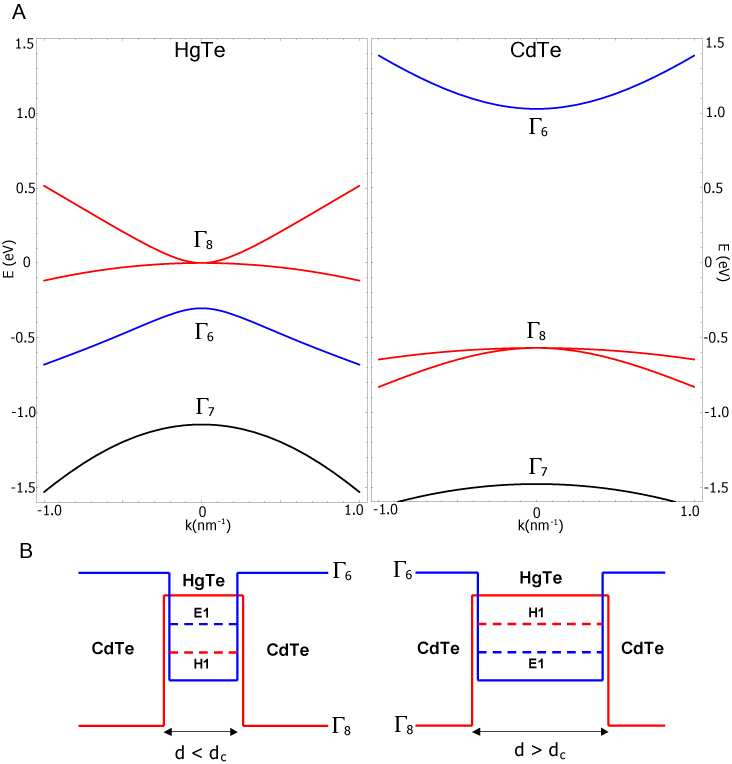
\includegraphics[width=0.95\linewidth]{quantum_well.png}
                \caption{Объемный спектр HgTe и CdTe и 
                         схематическое изображение квантовой ямы}
            \end{figure}
        \end{column}
        \begin{column}{0.5\textwidth}
            В квантовой яме образуются уровни размерного квантования. При
            $d < d_c$ спектр ямы нормальный, при $d > d_c$ --- 
            инвертированный.
            \begin{figure}
                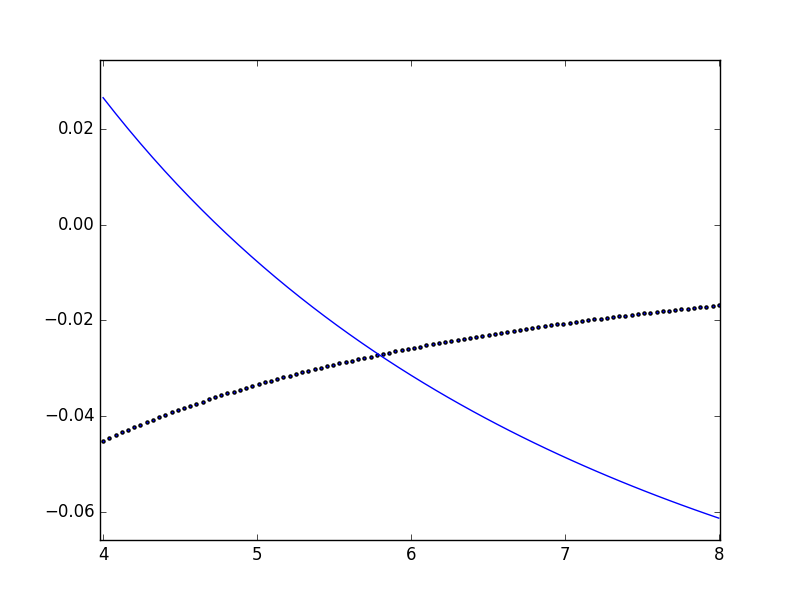
\includegraphics[width=0.95\linewidth]{levels.png}
                \caption{Уровни размерного квантования}
            \end{figure}
        \end{column}
    \end{columns}
\end{frame}

\begin{frame}
    \frametitle{Гамильтониан Кейна}
    \begin{equation}
        H = \begin{pmatrix}
                    E_c + \frac{\hbar^2 k^2}{2m_s}E_{2\times 2} & T \\
                    T^\dagger & E_v + H_{L}
            \end{pmatrix}
    \end{equation}
    \begin{multline*}
        H_L = -\frac{\hbar^2}{2m_0}\left[
                \left(\gamma_1 + \frac{5}{2}\gamma_2\right)k^2 -
                2\gamma_2(\vec{k} \cdot \vec{J})^2 - \right. \\
                - \left.2(\gamma_3 - \gamma_2)(\{J_x J_y\} + \{J_x J_z\} + \{J_y J_z\})
                \vphantom{\frac{1}{2}}\right]
    \end{multline*}
    \begin{equation*}
        T = P\begin{pmatrix}
               -\frac{1}{\sqrt{2}}k_{+} & \sqrt{\frac{2}{3}}k_z  
                        & \frac{1}{\sqrt{6}} k_{-} & 0 \\
                0 & -\frac{1}{\sqrt{6}} k_{+} 
                        & \sqrt{\frac{2}{3}}k_z & \frac{1}{\sqrt{2}} k_{-} 
             \end{pmatrix}
    \end{equation*}
\end{frame}

\begin{frame}
    \frametitle{Эффективный гамильтониан для уровней размерного квантования}
        Эффективный гамильтониан для E1, H1 подуровней квантовой ямы HgTe:
        \begin{equation}
           \label{eff_so_ham}
            \scalebox{0.6}{%
            $
            H = \left(\begin{matrix}
                    \xi + \frac{1}{m}(2 - \cos{p_x} - \cos{p_y}) & 
                            2t(\sin{p_x} - i\sin{p_y})   \\
                    2t(\sin{p_x} + i\sin{p_y}) & 
                           - \xi - \frac{1}{m}(2 - \cos{p_x} - \cos{p_y}) \\
                \end{matrix}\right)
            $
            }
        \end{equation}
        Описывает топологический изолятор при $\xi < 0$
\end{frame}

\begin{frame}
    \frametitle{Гамильтониан в координатном представлении}
    \begin{multline}
        \label{BHZ_tight_binding}
        H_{\mathrm{lattice}} = \sum_{mn} \left\{
            a_{mn}^\dagger\left( \left(\xi + \frac{2}{m}\right) a_{mn} \right.\right.\\
     \left.\left. -\frac{1}{2m}(a_{m+1,n} + a_{m-1,n} + a_{m,n+1} + a_{m,n-1})\right)\right. \\
            -it a_{mn}^\dagger(b_{m+1,n} -b_{m-1,n} - i(b_{m,n+1} - b_{m,n-1}))\\
            -it b_{mn}^\dagger(a_{m+1,n} -a_{m-1,n} + i(a_{m,n+1} - a_{m,n-1}))\\
            -\left. b_{mn}^\dagger\left( \left(\xi + \frac{2}{m}\right) b_{mn}
                     -\frac{1}{2m}(b_{m+1,n} + b_{m-1,n} + b_{m,n+1} + b_{m,n-1})\right) \right\}
    \end{multline}
\end{frame}
    

\begin{frame}
    \frametitle{Краевые моды}
    \begin{columns}[T]
        \begin{column}{0.5\textwidth}
            \begin{figure}[h]
                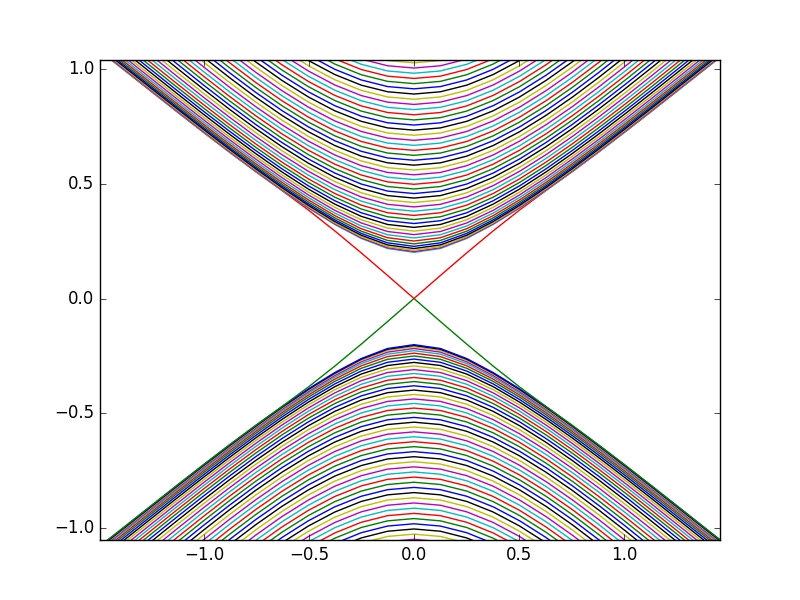
\includegraphics[width=0.95\linewidth]{edge_states.png}
                \caption{Спектр полосы ТИ: результат численной диагонализации}
            \end{figure}
        \end{column}
        \begin{column}{0.5\textwidth}
            На границе топологического изолятора образуются моды, пересекающие щель.
            Их закон дисперсии --- $\epsilon \approx \pm vk$ для двух проекций спина. 
            $T$--инвариантное возмущение не может привести к рассеянию краевых 
            электронов назад.
    
            Какие могут быть механизмы для рассеяния?
        \end{column}
    \end{columns}
\end{frame}

\begin{frame}
    \frametitle{Реконструкция края}
    \begin{columns}[T]
        \begin{column}{0.5\textwidth}
               \begin{figure}[h]
                   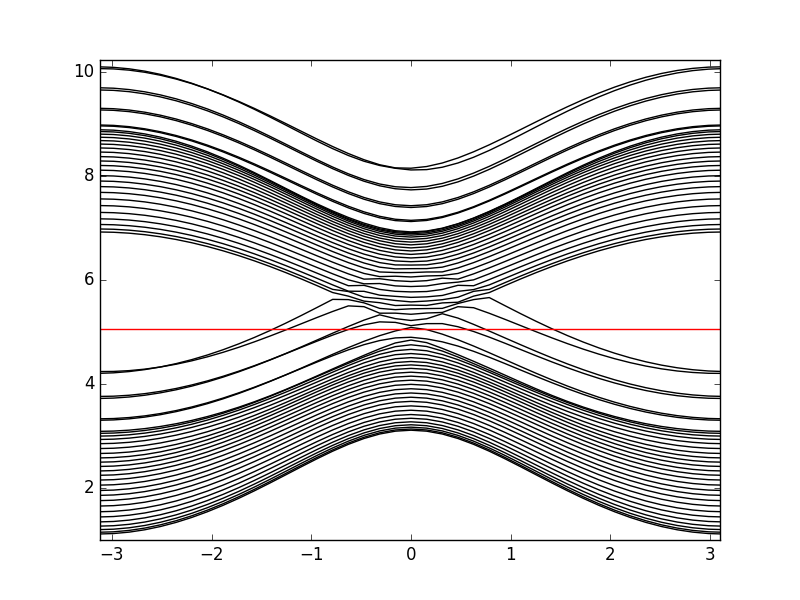
\includegraphics[width=0.99\linewidth]{reconstruction_spectrum_down.png}
                   \caption{Спин вниз}
               \end{figure}
        \end{column}
        \begin{column}{0.5\textwidth}
               \begin{figure}[h]
                   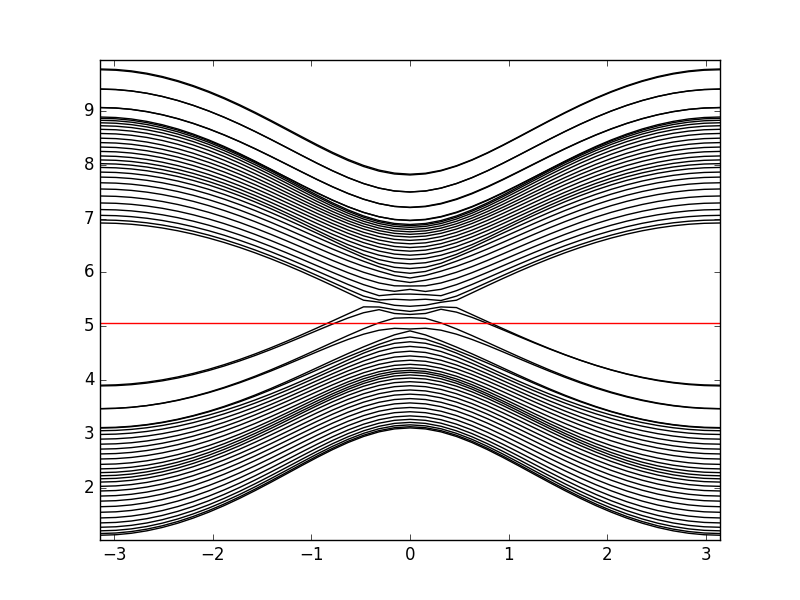
\includegraphics[width=0.99\linewidth]{reconstruction_spectrum_up.png}
                   \caption{Спин вверх}
               \end{figure}
        \end{column}
    \end{columns}
\end{frame}

\begin{frame}
    \frametitle{Точечная примесь}
    \begin{equation}
        V = \Delta E (a_{00}^\dagger a_{00} + b_{00}^\dagger b_{00})
    \end{equation}
    Уравнение на уровень энергии:
    \begin{equation}    
        \label{imp_equation}
        \det{\left(\mathbbm{1} - \Delta E \hat{G}(\omega, 0, 0)\right)} = 1,
    \end{equation}
    \begin{equation}    
        \label{green_function}
        \hat{G}(\omega, m, n) = \int \frac{d^2 p}{(2\pi)^2} e^{ip_x m + ip_y n}
                \frac{\omega + \hat{H}}{\omega^2 - E_p^2},
    \end{equation}
\end{frame}

\begin{frame}
    \frametitle{Уровни энергии на примеси}
    \begin{figure}[h]
        \centering
        \begin{minipage}[t]{0.45\linewidth}
            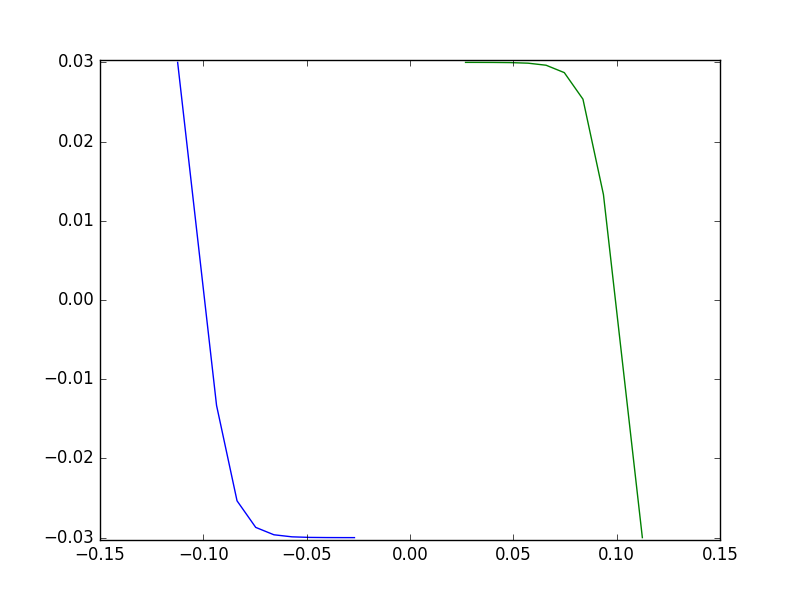
\includegraphics[width=0.99\linewidth]{impurity_levels.png}
        \end{minipage}
        \hfill
        \begin{minipage}[t]{0.45\linewidth}
            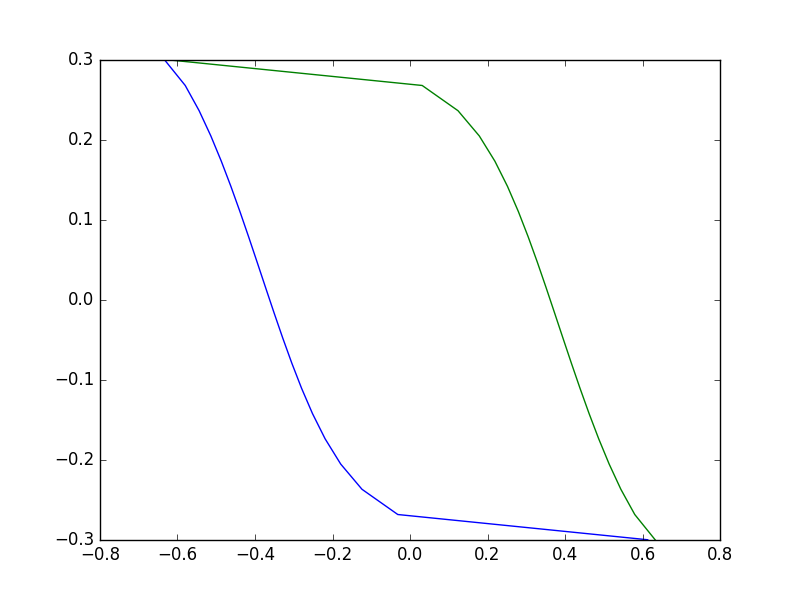
\includegraphics[width=0.99\linewidth]{gf_03-1-04.png}
        \end{minipage}
            \caption{
                    На графиках показаны уровни энергии связанных состояний на точечной примеси
                    для $m,t = 1,0.4$, $\xi = 0.03$ (слева), $\xi = 0.3$ (справа)
                    }
        \label{fig:impurity_numeric_levels}
    \end{figure}
\end{frame}

\begin{frame}
    \frametitle{Волновые функции}
    \begin{equation}
        \begin{split}
            G_{11}(\omega, m, n) & = -\frac{1}{2\pi} \frac{1}{4t^2 + \frac{\xi}{m}}
            \left( \omega + \xi - \frac{1}{m} \frac{\xi^2 - \omega^2}{4t^2 + \frac{\xi}{m}} \right)
            K_0 \left(\sqrt{\frac{\xi^2 - \omega^2}{4t^2 + \frac{\xi}{m}}}R \right)\\
            G_{21}(\omega, m, n) & = -\frac{it}{\pi} \sqrt{\frac{\xi^2 - \omega^2}
                                         {(4t^2 + \frac{\xi}{m})^{3}}}
            K_1 \left(\sqrt{\frac{\xi^2 - \omega^2}{4t^2 + \frac{\xi}{m}}}R \right)e^{i\theta}
        \end{split}
    \end{equation}
    \begin{equation} 
        \label{impurity_energy}
        \delta \omega \approx \frac{\left(4t^2 + \frac{\xi}{m}\right)p_{\mathrm{max}}^2}{|\xi|}
                \exp\left\{ -\frac{p_{\mathrm{max}}^2}{4m|\xi|} - 
                            \frac{2\pi}{|\xi|\Delta E\left(4t^2 + \frac{\xi}{m}\right)}\right\}
    \end{equation}
\end{frame}

\begin{frame}
    \frametitle{Результаты диагонализации}
    \begin{figure}[h]
        \centering
        \begin{minipage}[t]{0.4\linewidth}
            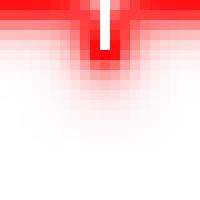
\includegraphics[width=0.9\linewidth]{obstacle_1.png}
        \end{minipage}
        \hfill
        \begin{minipage}[t]{0.4\linewidth}
            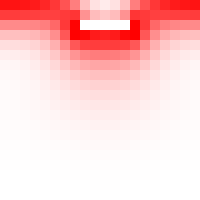
\includegraphics[width=0.9\linewidth]{obstacle_2.png}
        \end{minipage}
        \caption{
            Квадрат амплитуды волновой функции краевого состояния, огибающего препятствия. 
            Размер решётки --- $20\times20$, по горизонтальной оси наложены периодические
            граничные условия.
        }
        \label{fig:obstacle}
    \end{figure}
\end{frame}

\begin{frame}
    \frametitle{Результаты диагонализации}
    \begin{figure}[h]
        \centering
        \begin{minipage}[h]{0.4\linewidth}
            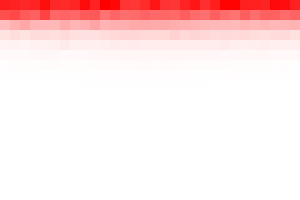
\includegraphics[width=1.\linewidth]{dis_edge_state_1.png}
            \caption{
                Волновая функция краевого состояния с беспорядком.
                Параметры модели: $\xi, m, t = -0.2, 1, 0.4$, сила беспорядка --- $0.5$.
                }
        \end{minipage}
        \hfill
        \begin{minipage}[h]{0.4\linewidth}
            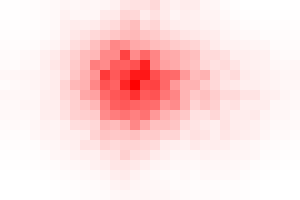
\includegraphics[width=1.\linewidth]{dis_bulk_state.png}
            \caption{
                Волновая функция объемного состояния с беспорядком для тех же параметров.
                }
        \end{minipage}
        \label{fig:disordered_stripe}
    \end{figure}
\end{frame}

\begin{frame}
    \frametitle{Результаты диагонализации}
    \begin{figure}[h]
        \centering
        \begin{minipage}[h]{0.9\linewidth}
            \centering
            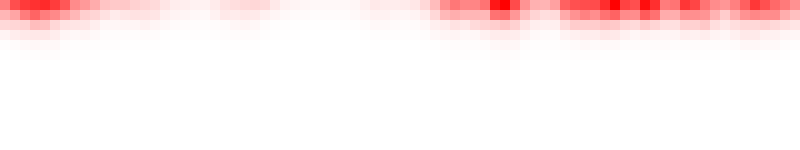
\includegraphics[width=0.7\linewidth]{mgn_edge_st_1.png}
        \end{minipage}
        \vfill
        \begin{minipage}[h]{0.9\linewidth}
            \centering
            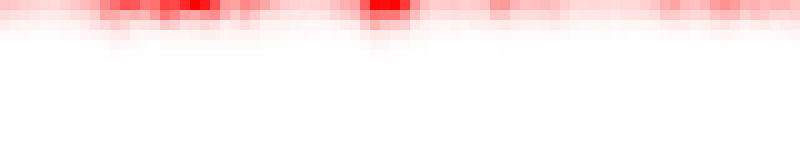
\includegraphics[width=0.7\linewidth]{mgn_edge_st_2.png}
        \end{minipage}
        \vfill
        \begin{minipage}[h]{0.9\linewidth}
            \centering
            
\includegraphics[width=0.7\linewidth]{mgn_edge_st_3.png}
        \end{minipage}
        \caption{
            Волновые функции краевых состояний с магнитным беспорядком 
            для тех же параметров.
            }
        \label{fig:magnetic_disorder}
    \end{figure}
\end{frame}
\begin{frame}
    \frametitle{Результаты диагонализации}
    \begin{figure}[h]
        \centering
        \begin{minipage}[h]{0.9\linewidth}
            \centering
            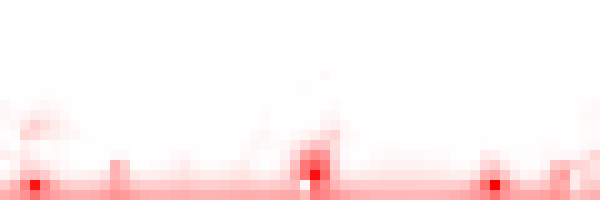
\includegraphics[width=0.7\linewidth]{fig4.png}
        \end{minipage}
        \vfill
        \begin{minipage}[h]{0.9\linewidth}
            \centering
            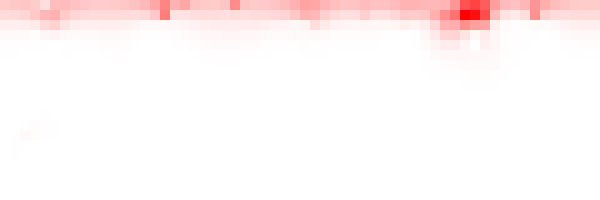
\includegraphics[width=0.7\linewidth]{fig5.png}
        \end{minipage}
        \vfill
        \begin{minipage}[h]{0.9\linewidth}
            \centering
            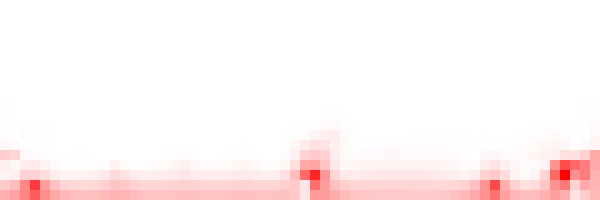
\includegraphics[width=0.7\linewidth]{fig6.png}
        \end{minipage}
        \caption{
            Волновые функции краевых состояний c примесями внутри щели      
        }
    
        \label{fig:magnetic_disorder}
    \end{figure}
\end{frame}
\end{document}
